\documentclass[oneside,a4paper]{refart}
\usepackage[svgnames]{xcolor}
\usepackage{genogram}
\usepackage{rotating, mathabx, multirow}
\usepackage{cleveref}

\newcommand{\pn}{\texttt{genogram}} %package name
\newcommand{\key}[1]{\texttt{\textcolor{OrangeRed}{#1}}}
\newcommand{\kitem}[1]{\item[\key{#1}\texttt{=\textcolor{Purple}{<value>}}]} %key item
\newcommand{\command}[1]{\textcolor{Blue}{\texttt{\char`\\#1}}}
\newcommand{\citem}[1]{\item[\command{#1}]} %command item
\newcommand{\default}[1]{\textcolor{ForestGreen}{\ttfamily#1}}
\newcommand{\intextmarginnote}[2][2pt]{\hspace*{-\marginparwidth}\hspace*{-\marginparsep}#2\\[#1]}
\crefname{figure}{Figure}{Figures}
\crefname{section}{Section}{Sections}

\newcommand{\versionnumber}{1.0}
\title{The \pn\ package: simply draw simple genograms}
\author{%
    \begin{tabular}{c}
        Alessandro Sciarra\\ {\small 22.03.2019}\\ \texttt{v\versionnumber}
    \end{tabular}
}

\date{}

\pagestyle{myheadings}
\markboth{The \pn\ package}%
         {The \pn\ package}

\makeindex

\setcounter{tocdepth}{2}
\settextfraction{0.85}

\begin{document}

\maketitle

\vspace{-1cm}
\begin{abstract}
        This document is meant to be a short reference manual
        for the \pn\ package. \emph{Usage simplicity} is
        the main goal of the package and, hence, just knowing which
        commands are available should suffice for most of the users.
\end{abstract}

The \pn\ is the result of a simple need: To provide an interface (as simple as possible) between the complex world of \texttt{pgf/TikZ} and \LaTeX\ newbies, which know just the basics\footnote{Indeed, it has been also a good opportunity for the author to study and deepen into the \texttt{pgfkeys} world, but this is not so relevant.}.
An example of what can be produced with this package is probably a good starting point to have an idea about it.
The Reader is then encouraged to have a look to \cref{fig:genogram} at \cpageref{fig:genogram}, where commands used to draw the genogram have also been included.

\section{Package usage}

Although it is not at necessary, you might consider to use this package in combination with the \texttt{standalone} class.
The idea behind this choice would be to produce a genogram to be then possibly included as figure in another document.
A minimal, to-be-completed example might be the following.
\begin{verbatim}
    \documentclass[border=1mm]{standalone}
    \usepackage{genogram}

    \begin{document}
        \drawGenogram
    \end{document}
\end{verbatim}
In \cref{sec:code} you can find a way more complete example.

\section{Setting up and drawing the genogram}\label{sec:comm}

The flow to construct the genogram is simple.
At first, information about the family elements has to be provided and, only at the end, the resulting genogram has to be drawn.
In a more \TeX -nichal language, there is a drawing command to be issued at the end, after all other commands will have been used to set up features of the genogram.
As you will see the genogram is centred around a couple (husband and wife) and it is possible to draw them, their children, parents and siblings only.

\subsection*{The command keys}

All commands to set up the genogram have one optional value that consists of a comma separated list of \texttt{key=<value>} elements, where sometimes the \texttt{=<value>} is not needed and it must not be specified.
Possible keys, which will be mentioned later in the command description are the following.
\begin{description}
    \kitem{age} It is used to add the age of the person in the genogram.
    \kitem{name} It is used to add the name of the person in the genogram.
    \kitem{status} Possible values are \texttt{married}, \texttt{not married}, \texttt{separated} or \texttt{divorced}. This key determines how the couples in the genogram are connected.
    \kitem{of} Possible values are \texttt{wife} or \texttt{husband}. Use this key to specify who the command you are using refer to.
    \item[\key{male} or \key{female}] It is used to specify the sex of the element the command you are using refers to.
    \item[\key{dead}] It is used to specify that the command you are using refers to a dead person.
\end{description}

If you need to use for some reason a comma or an equal sign in the value of a key, you must enclose the value in curly braces, e.g. \verb|name={Paul, Jean}|.

\subsection*{The main commands}

Commands are in general used to add elements to the genogram.
Their names are self-explanatory and the following list provide the missing piece of information: Which key can be passed to which command.

\begin{description}
    \citem{drawGenogram}
        This is probably the main command of the package, in the sense that it is responsible of drawing the genogram.
        Remember to use it only after having specified all family members, but do not forget to use it!
    \citem{wife[...]}
        Accepted keys are \key{age}, \key{name}, \key{status} and \key{dead}.
        By default, the sex of the wife is assumed to be female, but the key \key{male} may be specified\footnote{For completeness, also the \key{female} key is accepted, but it has no effect, unless it is specified after having given the \key{male} key. Definitely a contrived scenario.}.
    \citem{husband[...]}
        Completely analogue to the \command{wife} command, but the default sex is male.
    \citem{child[...]}
        Accepted keys are \key{age}, \key{name}, \key{male} or \key{female} and \key{dead}.
        Although the default sex is male, you are encouraged to explicitly specify the sex to make your genogram more readable.
        This command can and has to be repeated to specify more children.
        The order in which children are drawn is left to right respecting the order in which they have been specified.
    \citem{mother[...]}
        Accepted keys are \key{of}, \key{age}, \key{name}, \key{status} and \key{dead}.
        Use the \key{of} key to specify whether you are specifying the mother of the wife or of the husband.
        The same consideration about the sex done for the wife are valid for the mother.
    \citem{father[...]}
        Completely analogue to the \command{mother} command, but the default sex is male.
    \citem{sister[...]}
        Accepted keys are \key{of}, \key{age}, \key{name}, and \key{dead}.
        Use the \key{of} key to specify whether you are specifying a sister of the wife or of the husband.
        This command can and has to be repeated to specify more sisters.
        The same consideration about the sex done for the wife are valid for the sister.
    \citem{brother[...]}
        Completely analogue to the \command{sister} command, but the default sex is male.
\end{description}

\paragraph{Remarks:}
\begin{itemize}
    \item The wife and the husband are always drawn.
    \item It is not possible to draw a single parent.
          Providing either the \command{mother} or the \command{father} command only will make a basic element for the unspecified parent be drawn.
    \item The \key{status} key needs to be specified only for one of the two elements of a couple.
          If you specify it in both elements, the later will be applied.
    \item The order in which siblings are drawn is at the left of the husband and at the right of the wife respecting the order in which they have been specified.

\end{itemize}

\subsection*{A command to customise the genogram appearance}

Although spacing between the genogram elements is treated in a quite dynamic way, it might be needed to affect the disposition of members in it.
For this purpose, you can use the \command{setBeforeDrawing[...]} command which also accepts a comma separated list of \texttt{key=<value>} as optional argument.
In this case the \texttt{<value>} is expected to be a length, i.e. a number followed by a unit of measure among \texttt{cm}, \texttt{mm}, \texttt{ex}, \texttt{em}, \texttt{in}, \texttt{pt}, \texttt{bp}, \texttt{dd} and \texttt{pc}\footnote{You can refer e.g. to \texttt{https://tex.stackexchange.com/a/8337/128737} for the conversions.}.
Possible keys are the following.

\intextmarginnote{\key{space around age}:}
This key refers to the white space around all ages in the genogram (between the number and either the square or the circle). The default value is \default{1pt}.

\intextmarginnote{\key{generation distance}:}
This is the \emph{vertical} distance between the centre of the shapes belonging to contiguous generations (e.g. the couple and the children). The default value is \default{3cm}.

\intextmarginnote{\key{couple distance}:}
This is the \emph{horizontal} distance between the centre of the husband and wife shapes. The default value is \default{10em} if the couple has less than 2 children, otherwise it is \default{5em} times the number of children.

\intextmarginnote{\key{husband parents distance}:}
This is the \emph{horizontal} distance between the centre of the husband parents shapes. The default value is \default{5em} times the number of the husband siblings increased by $1$.

\intextmarginnote{\key{wife parents distance}:}
This is the \emph{horizontal} distance between the centre of the wife parents shapes. The default value is \default{5em} times the number of the wife siblings increased by $1$.

\intextmarginnote{\key{broken couple symbol height}:}
For separated or divorced couple, you can change the height of the correspondent symbol using this key. The default value is \default{1ex}.

\intextmarginnote{\key{broken couple symbol width}:}
For separated or divorced couple, you can change the width of the correspondent symbol using this key. The default value is \default{0.5ex}.



\begin{center}\rule{0.5\textwidth}{1pt}\end{center}

\begingroup\small\marginlabel{\textcolor{DarkBlue}{\underline{\textsc{Advanced}}:}}
To offer to more advanced users the possibility to customise a bit more the genogram, two other keys are offered.
In order to use them, some \texttt{TikZ} knowledge is required.
Just ignore them, unless you need to do something that is not achievable using the provided commands.
In that case, these keys might be the way to go.

The two keys \key{extra node feature} and \key{extra label feature} accept as value a comma separated list of \texttt{key=<value>} elements which are forwarded to a \texttt{TikZ} node.
This implies that such a list has to be specified in curly braces, e.g.
\begin{center}
    \ttfamily extra node feature=\string{text=red, fill=yellow\string}
\end{center}
will make the genogram element text (the age) be typeset in red on yellow background.
As you might have already guessed, the genogram element (square or circle with inside the age) is a \texttt{TikZ} node to which the key \key{extra node feature} refers.
The name of a person in the genogram is also a \texttt{TikZ} node and you can customise it using the \key{extra label feature} key.
At the moment there is no key to customise paths.

\endgroup


\newpage

\global\pdfpageattr\expandafter{\the\pdfpageattr/Rotate 90}
\begin{fullpage}
    \begin{sidewaysfigure}[ht]
        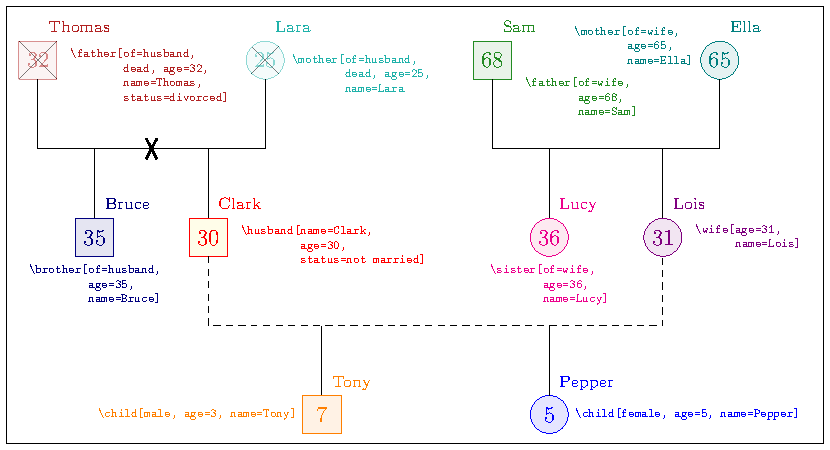
\includegraphics[width=\textwidth]{genogram_example}
        \caption{Demonstration of the \pn\ at work.}
        \label{fig:genogram}
    \end{sidewaysfigure}
\end{fullpage}
\global\pdfpageattr\expandafter{\the\pdfpageattr/Rotate 0}

\section{The code to produce \cref{fig:genogram} {\scriptsize(without printing commands)}}\label{sec:code}

\vspace{-4mm}
\begingroup\small

\marginlabel{\vspace{3.5mm} Black and white:}
\begin{verbatim}
  \documentclass[border=1mm, svgnames]{standalone}
  \usepackage{genogram}
  \begin{document}
      \husband[name=Clark, age=30, status=not married]
      \wife[age=31, name=Lois]
      \child[male, age=7, name=Tony]
      \child[female, age=5, name=Pepper]
      \mother[of=wife, age=65, name=Ella]
      \father[of=wife, age=68, name=Sam]
      \mother[of=husband, dead, age=25, name=Lara]
      \father[of=husband, dead, age=32, name=Thomas, status=divorced]
      \sister[of=wife, age=36, name=Lucy]
      \brother[of=husband, age=35, name=Bruce]
      \drawGenogram
  \end{document}
\end{verbatim}

%\vspace{-4mm}
\marginlabel{\vspace{3.6mm}Coloured version:}
\begin{verbatim}
  \documentclass[border=1mm, svgnames]{standalone}
  \usepackage{genogram}

  \begin{document}
      \husband[name=Clark, age=30, status=not married,
               extra node feature={red, fill=yellow!10},
               extra label feature={text=red}]
      \wife[age=31, name=Lois,
            extra node feature={violet, fill=violet!10},
            extra label feature={text=violet}]
      \child[male, age=7, name=Tony,
             extra node feature={orange, fill=orange!10},
             extra label feature={text=orange}]
      \child[female, age=5, name=Pepper,
              extra node feature={blue, fill=blue!10},
              extra label feature={text=blue}]
      \mother[of=wife, age=65, name=Ella,
              extra node feature={Teal, fill=Teal!10},
              extra label feature={text=Teal}]
      \father[of=wife, age=68, name=Sam,
              extra node feature={ForestGreen, fill=ForestGreen!10},
              extra label feature={text=ForestGreen}]
      \mother[of=husband, dead, age=25, name=Lara,
              extra node feature={LightSeaGreen, fill=LightSeaGreen!10},
              extra label feature={text=LightSeaGreen}]
      \father[of=husband, dead, age=32, name=Thomas, status=divorced,
              extra node feature={FireBrick, fill=FireBrick!10},
              extra label feature={text=FireBrick}]
      \sister[of=wife, age=36, name=Lucy,
              extra node feature={magenta, fill=magenta!10},
              extra label feature={text=magenta}]
      \brother[of=husband, age=35, name=Bruce,
               extra node feature={Navy, fill=Navy!10},
               extra label feature={text=Navy}]
      \drawGenogram
  \end{document}
\end{verbatim}
\endgroup

\newpage


\section{Towards more freedom \hfill{\color{DarkBlue}\normalfont\scshape Advanced}}

If you know \LaTeX\ as well as \texttt{TikZ} more than just a bit, you might be interested in adding more details to your genogram.
The \command{addToTikzpicture\string{...\string}} command has been added exactly for you\footnote{Indeed, the commands in \cref{fig:genogram} have been added exactly using this command.}!
Specifying it -- clearly before \command{drawGenogram} -- you can continue drawing in the \texttt{tikzpicture} freely, after that the genogram has been drawn.
It is enough to give valid \texttt{TikZ} code in its mandatory argument.
Available \texttt{nodes} are
\begin{center}
    \ttfamily
    \begin{tabular}{l@{\hspace{4em}}l@{\hspace{4em}}l}
        gen@husband              &  gen@wife            & \multirow{4}{*}{gen@child<n>}\\
        gen@husband@mother       &  gen@wife@mother     & \\
        gen@husband@father       &  gen@wife@father     & \\
        gen@husband@sibling<n>   &  gen@wife@sibling<n> & \\
    \end{tabular}
\end{center}
and the names as well as the positions should be self explanatory.
Note that \texttt{<n>} should be substituted with positive integers numbers and the index increases as the genogram elements are drawn.
For each of the above listed nodes, two additional \texttt{coordinates} exists and they are called \texttt{<node name>@above} and \texttt{<node name>@below}.
These coordinates refer to points exactly in the middle between generations.
\emph{If you know arrived here reading this section, you will know how to make use of this information.}



\end{document}
